\section{Diana Misiaczyńska\item \item }
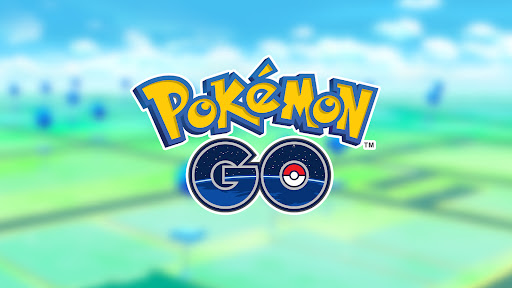
\includegraphics[width=12cm, height=5cm]{pictures/pokemon.jpg}   \newline
fajne pokemony:
\begin{itemize}
  \item eevee
  \item sunflora
  \item cherrim
  \item stunkfisk
  \item castform
\end{itemize}
\newline
\vspace{1.5cm}
też fajne:
\begin{enumerate}
  \item absol
  \item machoke
  \item oricorio
  \item wailmer
\end{enumerate}
\newline

Równanie kwadratowe posiadać może rozwiązanie w liczbach rzeczywistych, lub też może tego rozwiązania nie posiadać. Liczba rozwiązań równania kwadratowego zależy od wartości wyróżnika
\[ \Delta = b^2-4ac \] 

\newline

\begin{table}[htbp]
\begin{tabular}{|l|l|l|}
\hline
\textbf{pokemon} & \textbf{typ} & \textbf{CP} \\ \hline
rogacz           & bug          & 1650        \\ \hline
sunflora         & grass        & 1484        \\ \hline
solrock          & rock/psychic & 1491        \\ \hline
vaporeon         & water        & 1445        \\ \hline
\end{tabular}
\end{table}
Pokemon GO to stworzona przez studio \textbf{Niantic} gra RPG, która wykorzystuje technologię rozszerzonej rzeczywistości (Augmented Reality). Produkcja wykorzystuje \underline{wbudowaną w smartfony i tablety kamerę do rejestrowania obrazu}, a następnie nakłada na to elementy gry, takie jak Pokemony. Do poruszania się w świecie gry wykorzystywany jest system  \textbf{GPS} - gracz porusza się wzdłuż realnie istniejących ulic i odwiedza rozmaite punkty rozrzucone po świecie. Rozgrywka koncentruje się na łapaniu i trenowaniu Pokemonów, a następnie wykorzystywaniu ich do walki z innymi graczami. \par
W dniu premiery Niantic udostępniło ich \emph{pierwszą generację}, czyli aż 150 różnych Pokemonów rozsianych po całym świecie. Wiele z nich dostępnych jest jedynie na konkretnych kontynentach.


